% vim: set tw=0:
\documentclass{beamer}
\usepackage{graphicx}
\usepackage{hyperref}
\hypersetup{pdfborder={0 0 0 0}}

% Reasonable themes:
% Antibes Bergen Berkeley Berlin Frankfurt Goettingen Ilmenau Luebeck Malmoe
% Montpellier PaloAlto Rochester Singapore Szeged Warsaw bars boxes
% compatibility default lined plain shadow sidebar split tree
% And these ones include the author's name on every slide:
% Berkeley

% Declare themes.
\mode<presentation>
\usetheme{UWHEP}

% Personal macros.
\newcommand{\email}[1]{{\texttt #1}}
\newcommand{\newframe}[1]{\section{#1}
    \frametitle{\sc{#1}}}
\newcommand{\subframe}[1]{\subsection{#1}
    \frametitle{\sc{#1}}}
\newcommand{\supers}[1]{\ensuremath{^\textrm{#1}}}
\newcommand{\subs}[1]{\ensuremath{_\textrm{#1}}}
\newcommand{\ca}{\ensuremath{\sim}}
\renewcommand{\email}[1]{\href{mailto:#1}{\nolinkurl{#1}}}

% Author information.
\title{T2 Status}
\author[Maier, Mohapatra]{
    Will Maier \and Ajit Mohapatra\\
    {\tt wcmaier@hep.wisc.edu}\\
    {\tt ajit@hep.wisc.edu}}
\institute[Wisconsin]{University of Wisconsin - High Energy Physics}
\date{2010.02.02}
\logo{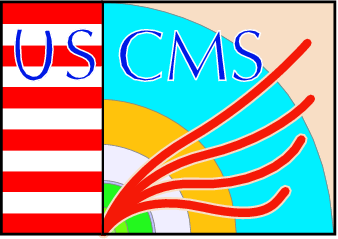
\includegraphics[height=0.6cm]{../../../Graphics/USCMS_logo.png}\hspace{.1cm}
\includegraphics[height=0.75cm]{../../../Graphics/UW_logo.png}}

\begin{document}

\begin{frame}
    \titlepage
\end{frame}

%\section{Overview}
%\begin{frame}
%    \tableofcontents
%\end{frame}

\section{Facilities}
\subsection{Software and Storage}
\begin{frame}
\frametitle{}

\begin{itemize}
	\item Ran into more {\tt OSM not found} errors in PNFS
	\begin{itemize}
		\item Breaks PNFS' linked lists of directories
		\item Given {\tt /a/b/c/d}, moving {\tt d} to {\tt /a} and then deleting {\tt b} causes the error
		\item Not sure about recovery\ldots{}
	\end{itemize}
	\item Running CRAB successfully on SL5 user interface machines
	\begin{itemize}
		\item Until opportunistic resources finish the upgrade, we'll keep our UI machines mostly SL4
	\end{itemize}
	\item Readying new release of {\tt pyCLI}~\footnote{\url{http://code.hep.wisc.edu/cli}}
	\begin{itemize}
		\item Basis for local {\tt dcache-tools}~\footnote{\url{http://code.hep.wisc.edu/dcache-tools}} package
		\item Switch from {\tt optparse} to {\tt argparse}, more unittests, compatible with Python 2.4-2.6 
	\end{itemize}
	\item More pool clean up
	\begin{itemize}
		\item Restored \ca{}20 TB of disk on broken hardware
	\end{itemize}
\end{itemize}
\end{frame}

\subsection{Production and Monitoring}
\begin{frame}
\frametitle{}

\begin{itemize}
	\item JobRobot: OK
	\item SAM: OK
	\item RSV: OK
	\item PhEDEx:
	\begin{itemize}
		\item No news
	\end{itemize}
	\item MC Production:
	\begin{itemize}
		\item Mike Anderson reports that production has been quiet, no issues
	\end{itemize}
\end{itemize}
\end{frame}

\end{document}
